\documentclass[12pt]{article}
\usepackage{cite}
\usepackage{fullpage}
\usepackage{graphicx}

\title{Progress Report Fall 2014}
\author{Robert Lowe}

\begin{document}
\maketitle

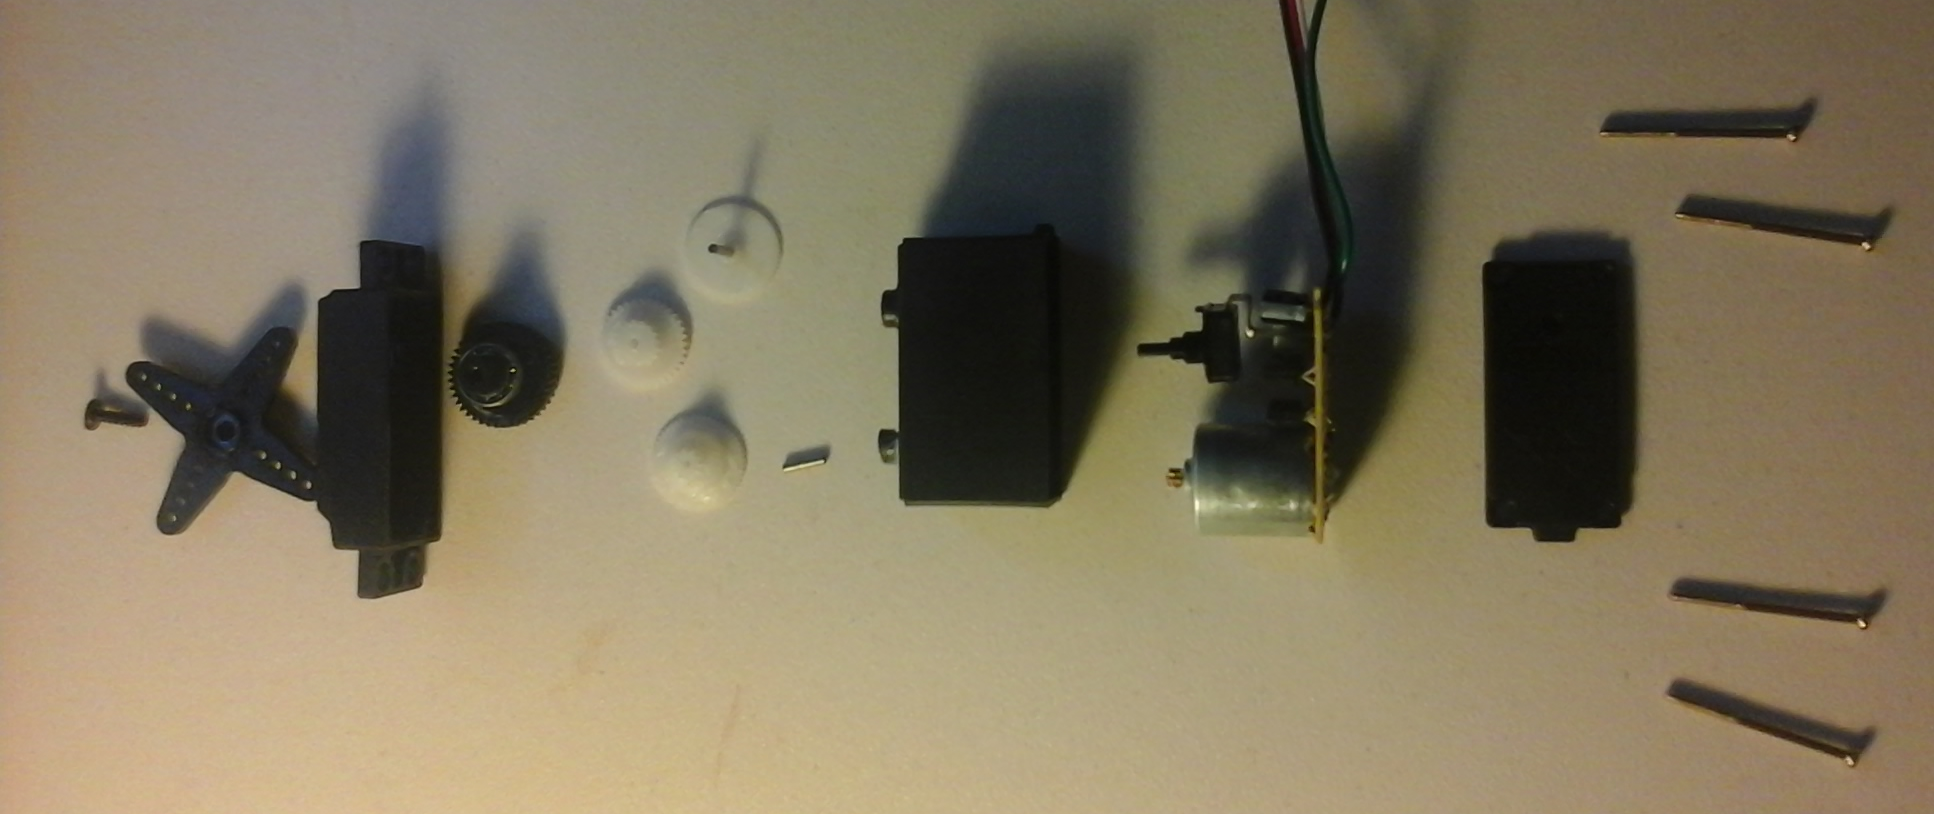
\includegraphics[width=\linewidth]{images/futabaExploded}
\section{Overview}
The basic story of this semester's progress is a frustrating tale of
trying to make steady progress through a series of fits and starts.
The largest obstacle has not been in technical challenges but rather
in scheduling.  On average, I was able to spend about 10 hours per
week on my research, which has resulted in slower progress than I
would have liked.

That being said, I did get quite a lot done when taking my schedule
obstacles into consideration.  The biggest component of this, as you
know,is that I have started working toward tenure during this
semester.  This is doubly compounded in that I am the only computer
scientist at Maryville College, and the semester that I joined the
faculty was during the time when the curriculum of the college was
under intense review.  So keep in mind that in addition to what has
been accomplished here, I have also authored changes to an entire
major as well as written a substantial portion of Maryville College's
core mathematical requirements.  (Not to mention teaching 9 hours,
managing the CS budget, travelling with the programming team, and
carrying out normal faculty committee type acivities!)

I attempted to divide my efforts between reading, writing, and
implementation activities.  The idea for this strategy is that I can
have a nice broad base going into the critical winter months, where I
will have much more time to work on research, with a fuller picture of
what I need to get done in order to advance my research as effeciently
as possible.  In so doing, I am beginning to see a glimmer of hope in
being able to complete this undertaking well in advance of the
deadline, after which I would  get the boot from Maryville.

The summary of the good news is this:
\begin{itemize}
  \item I have settled on a prognostic algorithm which fits
    both my needs and the current prognostic literature.
  \item I have identified a technique which shows promise in learning
    fault tolerant behaviors.
  \item I have completed the microcontroller level software that my
    test rig will need.
  \item I have been able to succesfully test data acquisition using my
    microcontroller, servo, and onboard computer set up.
  \item I am less intimidated, and even cautiosly optimistic, about
    the prospect of writing a bipedal gate generator.
  \item My literature review is taking shape, and I have adequate
    notes to start fleshing out my approach document.
\end{itemize}

\section{Reading Efforts}
My reading efforts for this semester have been spread across three
sections.  First, I have been reading a lot about bipedal walking
especially the inverted pendulum model, which is the model that I will
be using.  The second area of my reading has been in fault tolerant
systems with an emphasis on fault tolerant robots.  Finally, I have
reviewed the small amounts of literature which deal with self healing
systems, which is still emerging (and the subject of my own research).

\subsection{Bipedal Walking}
The papers I have read in bipedal walking are:
\begin{itemize}
  \item {\em The 3D Inverted Pendulum Mode: A Simple modeling for a
    biped walking pattern generation} by Shuuji Kajita et. al (2001).
  \item {\em A simple Reinforcement Learning Algorithm for Biped
    Walking} by June Morimoto et. Al (2004).
  \item {\em A simple trajectory Generation Method for Biped Walking}
    by Shuai Feng  and Zengqi Sun (2008)
  \item {\em Applying Neural Fields to the Stability Problem of an
    Inverted Pendulum as a Simple Biped Walking Model} by Juan
    Figuredo (2009)
\end{itemize}
Kajita's paper provides a base understanding for how the inverted
pendulum model works, and provided the needed details for me to
implement the model.  The other 3 papers provide various learning
tecniques for how gates can be parameterized and explored.  These will
be needed because I will be generating gates in response to failure
prognosis.

In addition to these, I have had to review various math and physics
textbooks in order to get abreast of the lagrangian mechanics of the
inverted pendulum model.

\subsection{Fault Tolerant Systems}
I read a few papers in the realm of fault tolerant systems.  This
builds on the papers I read over the summer.  There was not much which
I found applicable to what I am doing, but I did come across one paper
which I studied very closely, and which has given me many ideas about
how to proceed.  This paper was {\em Fast Damage Recovery in Robotics
  with the T-Reselience Algorithm} by Sylvian Koos and Antoine Cully
(2013).

This paper proivdes two helpful things.  First, they have a very
comprehensive overview of how damage recovery is traditionally
approached in robotics, and second they provide a hybrid approach
between two different methods of fault tolerance.  Their approach uses
a self-simulating robot which has a set of known responses to faults.
It then uses what the authors refer to as a ``transfer function'' to
decide what combination of the controllers to use.  This reduces the
number of parameters required to determine action in response to
failure, and allows for a fairly quick convergence when learning
responses to unknown failures.

I think that this algorithm could be modified to work with prognostic
parameters, and explore the search space of corrective actions so as
to avert and/or mitigate failure.


\subsection{Self-Healing Systems}
I did find some literature on self-healing systems, one of which was a
robotic paper.  There were two key papers which I studied:
\begin{itemize}
\item
\end{itemize}

\section{Writing Efforts}
\subsection{Approach Chapter}
\subsection{Literature Review Section}

\section{Implementation Efforts}
\subsection{Micrcontroller Code}
\subsection{Physical Implementation}
\subsection{Seeded Fault Tests}
\subsection{Particle Filter Prognostic Implementation}

\section{Next Steps}
\subsection{Coding Needs}
\subsection{Hardware Creation}
\subsection{Fault Seeding and Data Collection}
\subsection{Scheduling}
\end{document}
